\chapter{Experiments and Results}\label{chap:experiments}
In this chapter, we present a comprehensive analysis of the experiments conducted to compare our proposed method with the baseline approach, CutLER. We thoroughly evaluate both models across a diverse set of datasets to assess their performance. Additionally, we delve into the impact of training images containing overlapping instances, providing detailed quantitative results to illustrate how these images affect the model's performance. 

\section{Datasets}
For a fair comparison, we use the same datasets as the baseline for both training and evaluation. All models are trained on the ImageNet dataset and evaluated on a diverse set of benchmark datasets, including COCO, Pascal VOC, and KITTI. This ensures more consistent and comprehensive assessment of performance across different types of datasets.

\subsection{ImageNet}
The ImageNet dataset~\cite{deng2009imagenet} is a large-scale visual database designed for use in visual object recognition research. Developed by researchers at Princeton and Stanford, it contains more than 10,000,000 labeled images depicting 10,000+ object categories. Each image in the dataset is hand-labeled by humans, making it a valuable resource for training and benchmarking deep learning models in computer vision.

We generate MaskCut annotations for all images on the subset of ImageNet containing the 1000 categories and 1.3 million images (ImageNet-1K), which serve as the pseudo-ground truth for our experiments. Both the baseline method (CutLER) and our proposed method are trained on the ImageNet dataset. However, in the proposed method, a fraction of images are excluded during the mask-filtration process (images with no annotaions are removed).

\subsection{COCO}
The COCO (Common Objects in Context) dataset~\cite{lin2015microsoftcococommonobjects} is a widely-used benchmark in the field of computer vision, designed to spur advancements in object detection, segmentation, and captioning. It contains over 200,000 images with more than 80 object categories, annotated with precise bounding boxes, segmentation masks, and context-related captions. 

We use the validation set of the COCO 2017 split, which contains 5,000 images, for evaluating the models. Both bounding box coordinates and segmentation annotations are utilized as ground truths for evaluation.

\subsection{PASCAL VOC}
The PASCAL VOC 2012 dataset is a widely recognized benchmark in visual object recognition, comprising 11,530 images across 20 categories with comprehensive annotations for object detection, classification, and segmentation tasks. For evaluation, we use both the training and test images from the PASCAL VOC dataset and detailed bounding box annotations as ground truths.

\subsection{KITTI}
The KITTI dataset~\cite{Geiger2013IJRR} is a prominent benchmark for evaluating performance in autonomous driving and computer vision tasks, including object detection, tracking, and scene flow. It features high-resolution images captured from a stereo camera setup mounted on a moving vehicle, encompassing a variety of urban and rural driving scenarios. 

Although the KITTI dataset offers rich annotations, including 3D object labels and depth information, our evaluation focuses solely on bounding boxes. Since the dataset does not provide segmentation annotations, we utilize only the bounding box data to evaluate 7521 images from KITTI’s trainval split.

\subsection{Comic and Watercolor}
In addition to real-world image datasets, we also incorporate art datasets, such as Comic and Watercolor~\cite{Inoue_2018_CVPR}, to evaluate the model's generalization capabilities across diverse visual styles. Since these datasets lack segmentation annotations, we use only the bounding box data for evaluation.

\section{Metrics}
We mostly use precision metrics to evaluate the performance of the models in our work. This includes metrics like AP and AP50, which are standard metrics used in object detection and instance segmentation tasks to evaluate the performance of models. These metrics provide a measure of how good a model is at correctly identifying and localizing objects within an image.

\subsection{Average Precision}
Average Precision (AP) is a metric that summarizes the precision-recall curve, which plots precision against recall at different confidence thresholds. Precision is defined as the ratio of True Positive (TP) detections to the sum of True Positive and False Positive (FP) detections, while recall is the ratio of True Positive detections to the sum of True Positive and False Negative (FN) detections. Precision and Recall is defined as Eq.~\ref{eq:precision} and Eq.~\ref{eq:recall} respectively.

\begin{equation}
\label{eq:precision}
    P = \frac{TP}{TP + FP}
\end{equation}

\begin{equation}
	\label{eq:recall}
	R = \frac{TP}{TP + FN}
\end{equation}

The AP is calculated as the area under the precision-recall curve, which is typically computed using a numerical approximation method like the trapezoidal rule. It can be formally defined as Eq.~\ref{eq:avg_precision}, where \(n\) refers to different recall levels and \(R_n\)​ and\(P_n\)​ are the recall and precision at the \(n^{th}\) threshold.

\begin{equation}
	\label{eq:avg_precision}
	\text{AP} = \sum_{n=1}^{N} (R_n - R_{n-1}) \cdot P_n
\end{equation}

AP is typically averaged over multiple IoU thresholds. In our case, AP is averaged over IoU thresholds from 0.5 to 0.95 with a step size of 0.05.

\subsubsection{AP50}
AP50 is a specific case of the Average Precision metric, where the Intersection over Union (IoU) threshold is set to 0.50. IoU is a measure of the overlap between the predicted bounding box and the ground truth bounding box, defined as Eq.~\ref{eq:iou}.

\begin{equation}
	\label{eq:iou}
	IoU = \frac{\text{Area of Overlap}}{\text{Area of Union}}
\end{equation}

AP50 calculates the AP but only considers a detection as a true positive if the IoU between the predicted bounding box and the ground truth is greater than or equal to 0.50. This metric is useful for understanding how well a model can detect objects with a certain level of spatial accuracy.

\subsection{Average Recall}
Average Recall (AR) is a metric that measures the recall of a model averaged over multiple IoU thresholds. It quantifies how much of ground truth labels were accurately predicted by the model. It is a valuable metric for unsupervised detection as it does not penalize the models for detecting novel objects which are unlabeled in the dataset. The formula for AR is given by Eq.~\ref{eq:avg_recall}.

\begin{equation}
	\label{eq:avg_recall}
	AR = \frac{1}{|T|} \sum_{t \in T} R(t)
\end{equation}


where \( T \) is the set of IoU thresholds and \( R(t) \) is the recall (Eq.~\ref{eq:recall}) at a specific IoU threshold \( t \). In our case, AR is averaged over IoU thresholds from 0.5 to 0.95 with a step size of 0.05. 

\subsubsection{AR100}
AR100 (AR@100) is a variant of Average Recall that limits the number of detections per image to a maximum of 100. It represents the recall averaged across a range of IoU thresholds, constrained to 100 predictions per image. The formula for AR@100 is given by Eq.~\ref{eq:avg_recall_100}.

\begin{equation}
	\label{eq:avg_recall_100}
	AR100 = \frac{1}{|T|} \sum_{t \in T} R_{100}(t)
\end{equation}

where \( R_{100}(t) \) is the recall at IoU threshold \( t \), considering up to 100 detections per image. We use AR100 metric to compare recalls of the baseline and our model in Section~\ref{section:persistant_recall}.

\section{Implementation Details}
\label{section:implementation_details}
Our implementation largely follows the baseline approach; however, it is important to note a key difference in our setup. While in the baseline paper experiments use a batch size of 16, we utilize batch sizes of 4 and 8 due to resource constraints. To ensure a fair comparison, we also train the baseline model from scratch using these same batch sizes of 4 and 8. All our experiments follow the following setting. If there are some modifications, it would be mentioned in the respective sections.

\subsection{Training Data}
Only the images from ImageNet dataset (1.3 Million images) are used for the initial training and self-training. We do not use any supervised pre-trained models or labels for training baseline or the proposed method. However, the bounding box annotations are used to analyze the impact of images with overlapping instances and object-centric prior in Sections~\ref{section:overlap_experiment} and~\ref{section:obj_centic_prior_exp} respectively.

\subsection{MaskCut}

We apply MaskCut with N=3, generating up to three masks per image through repeated N-Cut operations, on images resized to 480×480 pixels to create pseudo-ground truths. The value of N is optimal at 3 for generating best quality masks for ImageNet dataset~\cite{wang2023cut}. The patch-wise affinity matrix generated from the key descriptors of the ViT-B/8 DINO model is used to perform the N-Cut operation. Additionally, we employ Conditional Random Fields (CRF)~\cite{sutton2010introductionconditionalrandomfields} to refine the masks and extract their bounding boxes.

\subsection{Detector}
Although CutLER is designed to be agnostic to the choice of object detector, we chose to use Cascade Mask R-CNN for all our experiments. This decision is based on the baseline paper's findings, which demonstrated that Cascade Mask R-CNN outperforms Mask R-CNN. We train the detector on ImageNet with MaskCut pseudo masks and bounding boxes for 160K iterations with a batch size of 4 or 8. 

The Copy-Paste augmentation is also used during the training process to improve robustness of object detection and segmentation models by exposing them to a wider range of scenarios and object contexts. In order to detect small objects, instead of vanilla copy-paste augmentation, masks are randomly downsampled with a scalar uniformly sampled between 0.3 and 1.0. 

We optimize the Detector using Stochastic Gradient Descent (SGD) for 160K iterations with a learning rate of 0.005, weight decay of \(5×10^{−5}\) and a momentum of 0.9. Training follows a learning rate schedule which decreases it by 5 after 80K iterations.

\subsection{Self Training}
In the baseline, at each stage, along with CutLER mask predictions with confidence score > 0.7 generated using the model from the previous stage, Maskcut masks which have IoU < 0.5 with the CutLER prediction masks together make the pseudo-ground truth masks for that stage. This has already been explained in detail in Section~\ref{section:proposed_mask_filtration_self_training}. The detector is then optimized using SGD with a learning rate of 0.01 over 80,000 iterations. We do not employ DropLoss during these self-training phases just as in the baseline.

\subsection{Resources}
Generating MaskCut annotations for all images in ImageNet is supposed to be the most time consuming part. But we used the pre-generated MaskCut annotations to save time.

Initial training on ImageNet with batch size 8 spans over 160K iterations on four NVIDIA rtx-2080 gpus takes around 1 day 18 hours and self-training of 80K iteration takes around 21 hours. The Training using filtered MaskCut masks generated by our method takes 4 hours less (1 day 14 hrs) as around 130K images are dropped in the mask filtration step for not having any pseudo-ground truth masks.


Filtered non-overlapping instance images and object-centric images representing only 35\% and 30\% of the ImageNet dataset, respectively, could be processed more efficiently compared to the baseline. Both methods require only approximately 18 hours for training.

\section{Experiments}
\subsection{Exploring the Impact of Overlapping Instances}
\label{section:overlap_experiment}
In this section, we describe the experiments conducted to evaluate the performance of the approaches mentioned in Section~\ref{section:analysis_ol_instancs}. ie, 1) Using all images of ImageNet (same as the baseline). 2) Using images without any overlapping instances, 3)  Only using images with overlapping instances. The primary goal is to assess how the presence or absence of overlapping instances in the training data influences the performance of the CutLER model. But we exclude approach 3 as we have insufficient images satisfying the condition (6\% of the annotated dataset), hence a fair comparison is not possible.

\subsubsection{Dataset}
We use the ImageNet dataset for training, focusing on the subset with ground truth bounding box annotations. For training the baseline, entire ImageNet dataset is used and doesn't use any bounding box annotations. 

For our approach, we utilize the annotated subset of ImageNet, which comprises 38\% of the entire dataset. Within this subset, we filter out images with overlapping instances where the IoU exceeds 0.1, based on the bounding box annotations. This filtering process drops 6\% of images from the annotated subset. Consequently, our approach utilizes only 35\% of the images employed by the baseline. It's important to note that while bounding box annotations are used solely for filtering images, the training process itself remains unsupervised, just like the baseline.

We evaluate our approaches and the baseline using the COCO 2017 Validation dataset, which contains 5,000 images spanning 80 different classes. Precision is calculated based on both bounding box and segmentation ground truths. To gain deeper insights, we further split the evaluation dataset into two subsets: images with overlapping instances and those without. This allows us to better analyze whether training without images that contain overlapping instances can improve the model's ability to distinguish individual instances in images where overlap occurs. Given the diverse range of images in the COCO 2017 Evaluation dataset, the split between images with and without overlapping instances is more balanced compared to ImageNet, with 48\% of the images containing overlapping instances and 52\% without. This balanced split ensures a fair and comprehensive comparison between our approach and the baseline.

\subsubsection{Training Procedure}
The training procedure for both the baseline and our proposed methods follow the standard CutLER training pipeline. MaskCut mask annotations serve as the pseudo-ground truth, and a Cascade Mask R-CNN is employed as the detector. Training is conducted incorporating Copy-Paste augmentations and DropLoss with batchsize 4 and 8 to minimize resource requirements. The baseline is trained over 160K iterations, while our methods to analyze the impact of overlapping instances and object-centric prior require only 80K iterations due to the smaller dataset size. This adjustment reflects the reduced training data in our approach, allowing for a more efficient training process without compromising the effectiveness of the model.

\begin{table}[htbp]
	\centering
	\begin{tabular}{c|cc|cc}
		\toprule
		\multirow{2}{*}{Metric} & \multicolumn{2}{c|}{Baseline} & \multicolumn{2}{c}{Ours} \\ \cmidrule{2-5}
		& AP & AP50 & AP & AP50 \\ \midrule
		bbox & 10.74 & 19.78 & \textbf{11.52} & \textbf{20.67} \\
		\midrule
		segm & 8.2 & 16.62 & \textbf{8.80} & \textbf{17.47} \\
		\bottomrule
	\end{tabular}
	\caption[\textbf{Evaluation of Models Trained With and Without Overlapping Instances }]{\textbf{AP and AP50 for Object Detection and Instance Segmentation Tasks} on COCO validation set using models trained (without self-training) on all images and images without overlapping instances}
	\label{tab:overlap_analysis}
\end{table}

\begin{table}[htbp]
	\centering
	\begin{tabular}{c|c|cc|cc}
		\toprule
		\multirow{2}{*}{COCO Val} & \multirow{2}{*}{Metric} & \multicolumn{2}{c|}{baseline} & \multicolumn{2}{c}{Ours} \\ \cmidrule{3-6}
		& & AP & AP50 & AP & AP50 \\ \midrule
		\multirow{2}{*}{All images} & bbox & 10.74 & 19.78 & \textbf{11.52} & \textbf{20.67} \\ 
		& segm & 8.2 & 16.62 & \textbf{8.80} & \textbf{17.47}  \\ \midrule
		\multirow{2}{*}{No overlapping instances} & bbox & 23.45 & 38.11 & \textbf{24.77} & \textbf{39.46} \\
		& segm & 19.19 & 35.19  & \textbf{20.13} & \textbf{36.36} \\
		\midrule
		\multirow{2}{*}{Only overlapping instances} & bbox & 7.25 & 15.11 & \textbf{8.52} & \textbf{16.8} \\ 
		& segm & 5.12 & 11.55 & \textbf{6.18} & \textbf{13.27} \\
		\bottomrule
	\end{tabular}
	\caption[\textbf{Evaluation of Models Trained With and Without Overlapping Instances With Evaluation Dataset Split}]{\textbf{AP and AP50 for Object Detection and Instance Segmentation Tasks Evaluated on Split COCO Validation Set} using models trained (without self-training) on all images and images without overlapping instances}
	\label{tab:combined_overlap_eval}
\end{table}

\subsubsection{Results}
\label{section:overlapping-results}
Even though the dropped images with overlapping instances are only 5\% of the annotated ImageNet subset, there is a notable improvement in the results. As it can be observed from Table~\ref{tab:overlap_analysis}, our method improves in both object detection and instance segmentation tasks. The table shows AP and AP50 of both object detection (bbox) and instance segmentation (segm) tasks on COCO validation set evaluated using the baseline and our approach. Even though the experiment is conducted using batch size 4, the results are still comparable to the baseline and model trained using our proposed mask filtration method (will be explained later in Section~\ref{section:mask_refinement_experiment}) with batch size 8, which can be observed from Table~\ref{tab:combined_train}. It is to be noted that the evaluation is performed using class-agnostic annotation generated from the original COCO annotations. We reuse the same annotation file used in CutLER.

To gain deeper insights, we further split the evaluation dataset into two subsets: images with overlapping instances and those without. It is to observe to what extent our approach helps to detect individual instances from images with overlapping instances. Results can be observed from Table~\ref{tab:combined_overlap_eval}. As anticipated, the evaluation scores for images with overlapping instances are significantly lower compared to those for images without overlaps. This disparity is likely due to the inherent challenge of grouping of instances when they overlap. Despite this challenge, it is noteworthy that both splits - images with and without overlapping instances showed a nearly equal improvement in performance for instance detection and segmentation tasks. This suggests that our approach is effective across different scenarios, affirming the model’s ability to generalize even in complex cases where instances are closely packed or overlapping.

\subsubsection{Improvement Across Classes}
\begin{figure*}
	\centering
	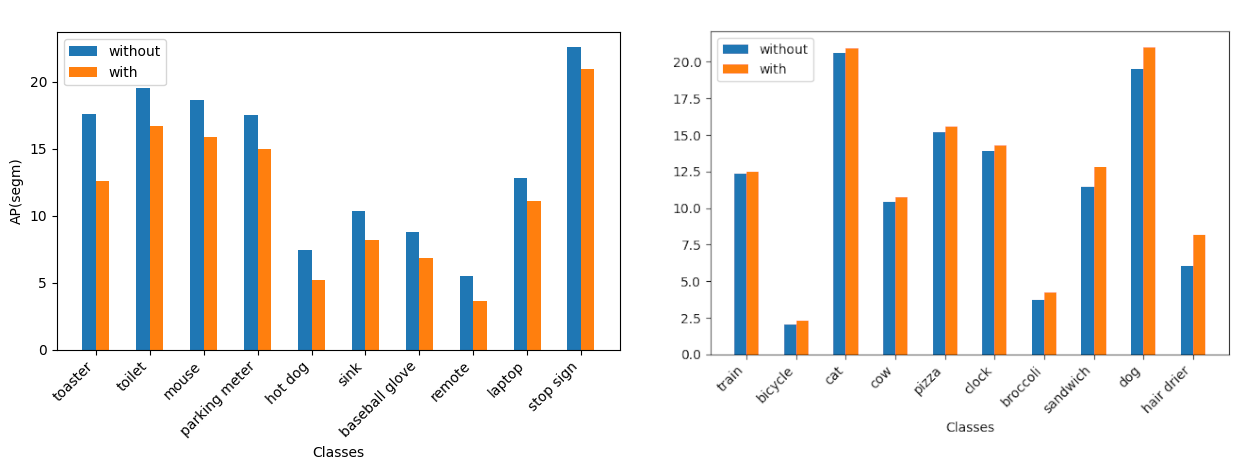
\includegraphics[width=1.05\textwidth]{Images/main/overlap_classes_new.png}
	\caption[\textbf{Training Without Overlapping Instances - Class-wise Comparison}]{\textbf{Class-wise Comparison} of change in \(AP_{segm}\) of models trained using images with and without overlapping instances evaluated on COCO validation set - 10 most and least improved classes}
	\label{fig:overlap_classes}
\end{figure*}

\begin{figure*}
	\centering
	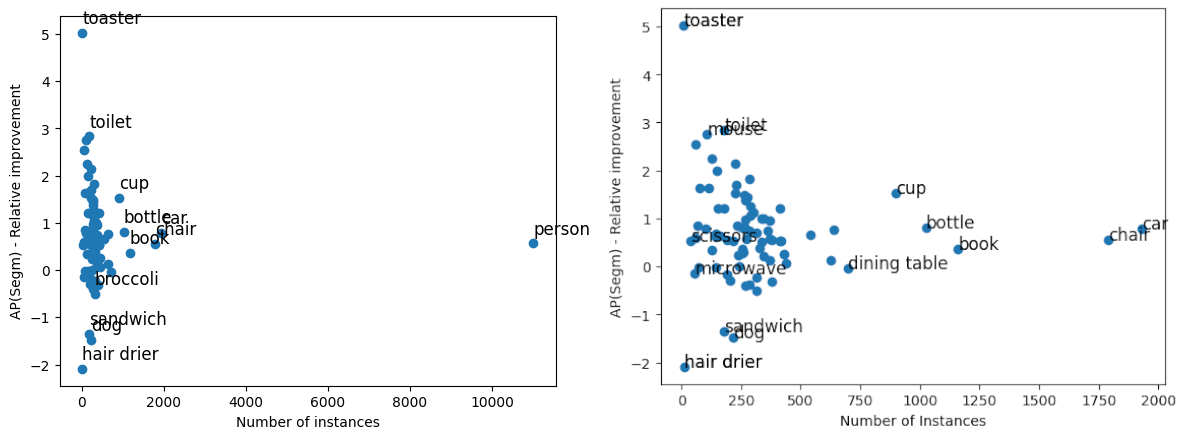
\includegraphics[width=1\textwidth]{Images/main/relative_improvement_combined.png}
	\caption[\textbf{Relative Improvement Against Number of Instances}]{\textbf{Relative Improvement (AP (Segm) ) Across Classes Against Number of Instances.} Relative improvement of our model against the baseline on the y-axis and number of instances on the x-axis. Classes corresponding to the extreme data points are highlighted. The plot on the right excludes the class \textbf{person} to make the analysis easier and more focused on the remaining classes.}
	\label{fig:relative_improvement}
\end{figure*}

To ensure that the observed improvements in performance were not simply due to the loss of accuracy in one class being offset by gains in another, class-wise improvements are calculated on the COCO validation set. This analysis allows for a more granular understanding of the model’s performance across different classes. By evaluating each class individually, we can verify that the enhancements in instance detection and segmentation are consistent and not merely the result of compensatory effects between classes. This class-wise assessment provides a clearer picture of the model's true capabilities, ensuring that the overall performance gains are robust and evenly distributed across the dataset.

The test results are illustrated in Fig.~\ref{fig:overlap_classes}, which highlights the 10 classes with the most significant improvements and the 10 classes with the least improvements evaluated on COCO validation set, based on the Average Precision for instance segmentation. Notably, our approach outperforms the baseline across the majority of classes. Specifically, it performs better in 68 out of the 80 classes assessed. In contrast, for the remaining 12 classes, our method shows reduced performance relative to the baseline.

To provide more clarity, we plot the relative improvement of our model over the baseline against the number of instances per class (Fig.~\ref{fig:relative_improvement}). This allows us to explore any potential correlation between the number of instances and the observed relative improvement. It can be observed that most classes with higher number of instances provide consistent improvement whereas classes with few instances are rather unpredictable. It underscores the effectiveness of our approach in enhancing instance segmentation performance across a broad range of classes, with only a few exceptions where it falls short.

\subsection{Exploring the Impact of Object-Centric Prior}
\label{section:obj_centic_prior_exp}
In this section, we describe the experiments conducted to evaluate the performance of the approaches mentioned in Section~\ref{section:analysis_oc_instancs}. ie, 1) Using all images of ImageNet 2) Only using object-centric images. We follow the same training procedure as the Experiment~\ref{section:overlap_experiment}. Hence it won't be explained again in this section.

\subsubsection{Dataset}
We use the ImageNet dataset for training focusing on the subset with ground truth bounding box annotations. We  also use the annotated subset of ImageNet, which comprises 38\% of the entire dataset. After filtration, we only use 30\% of the images employed by the baseline, which is even 5\% lesser images compared to Experiment~\ref{section:overlap_experiment}. It is due to removing the multi-instance images from the dataset. We use the same baseline as the Experiment~\ref{section:overlap_experiment} for comparison and the models are evaluated on all images of COCO validation set.

\subsubsection{Results}
As it can be observed from Table~\ref{tab:object-centric-analysis}, our method improves in both object detection and instance segmentation tasks. The table shows AP and AP50 of both instance detection and instance segmentation tasks on COCO validation set evaluated using the baseline and our approach.
\begin{table}[htbp]
	\centering
	\begin{tabular}{c|cc|cc}
		\toprule
		\multirow{2}{*}{Metric} & \multicolumn{2}{c|}{Baseline} & \multicolumn{2}{c}{Ours} \\ \cmidrule{2-5}
		& AP & AP50 & AP & AP50 \\ \midrule
		bbox & 10.74 & 19.78 & \textbf{11.32} & \textbf{20.43} \\
		\midrule
		segm & 8.2 & 16.62 & \textbf{8.62} & \textbf{17.43} \\
		\bottomrule
	\end{tabular}
	\caption[\textbf{Evaluation of Baseline vs Model Trained With Only Object-Centric Images}]{\textbf{AP and AP50 Bounding Box and Segmentation Evaluation} on COCO validation set with baseline and model trained using only object-centric images}
	\label{tab:object-centric-analysis}
\end{table}
Even by using only 30\% of the training data, we could obtain comparable results with the baseline. However, the model trained without overlapping instances (Experiment~\ref{section:overlap_experiment}) outperforms this method by a small margin.

\subsection{Proposed Mask Filtering Method}
\label{section:mask_refinement_experiment}
To address the issue of unwanted background masks included in the pseudo-ground truths, we introduce an enhanced mask filtration approach in Section~\ref{section:proposed_method}. This section details the experimental setup and results associated with our improved mask filtration technique.

\subsubsection{Dataset}
We use the ImageNet dataset for training and evaluate on COCO, KITTI, PASCAL VOC 2012, Comic and Watercolor datasets. During the initial phase of training, both the baseline and our proposed method utilize the full set of images from ImageNet. However, after the first round of mask filtration in our method, approximately 10\% of the images are discarded due to the absence of usable masks. Consequently, the corresponding MaskCut annotations for these excluded images are also removed and the remaining 90\% images constitute the training dataset for the self-training stage.

\subsubsection{Training Procedure}
The baseline follows the training procedure as described in Section~\ref{section:implementation_details}. But our method comes with one extra step of refining MaskCut masks using our modified mask filtration method explained in Section~\ref{section:proposed_method} and training from scratch again. This is followed by self-training as employed in the baseline to improve the performance further. We train both models using 4 and 8 batch sizes to analyze the influence of batch size on performance of the model (Section~\ref{section:choice_of_batch_size}). 

\subsubsection{Initial Training Phase: Mask Filtration}
\begin{figure*}
	\centering
	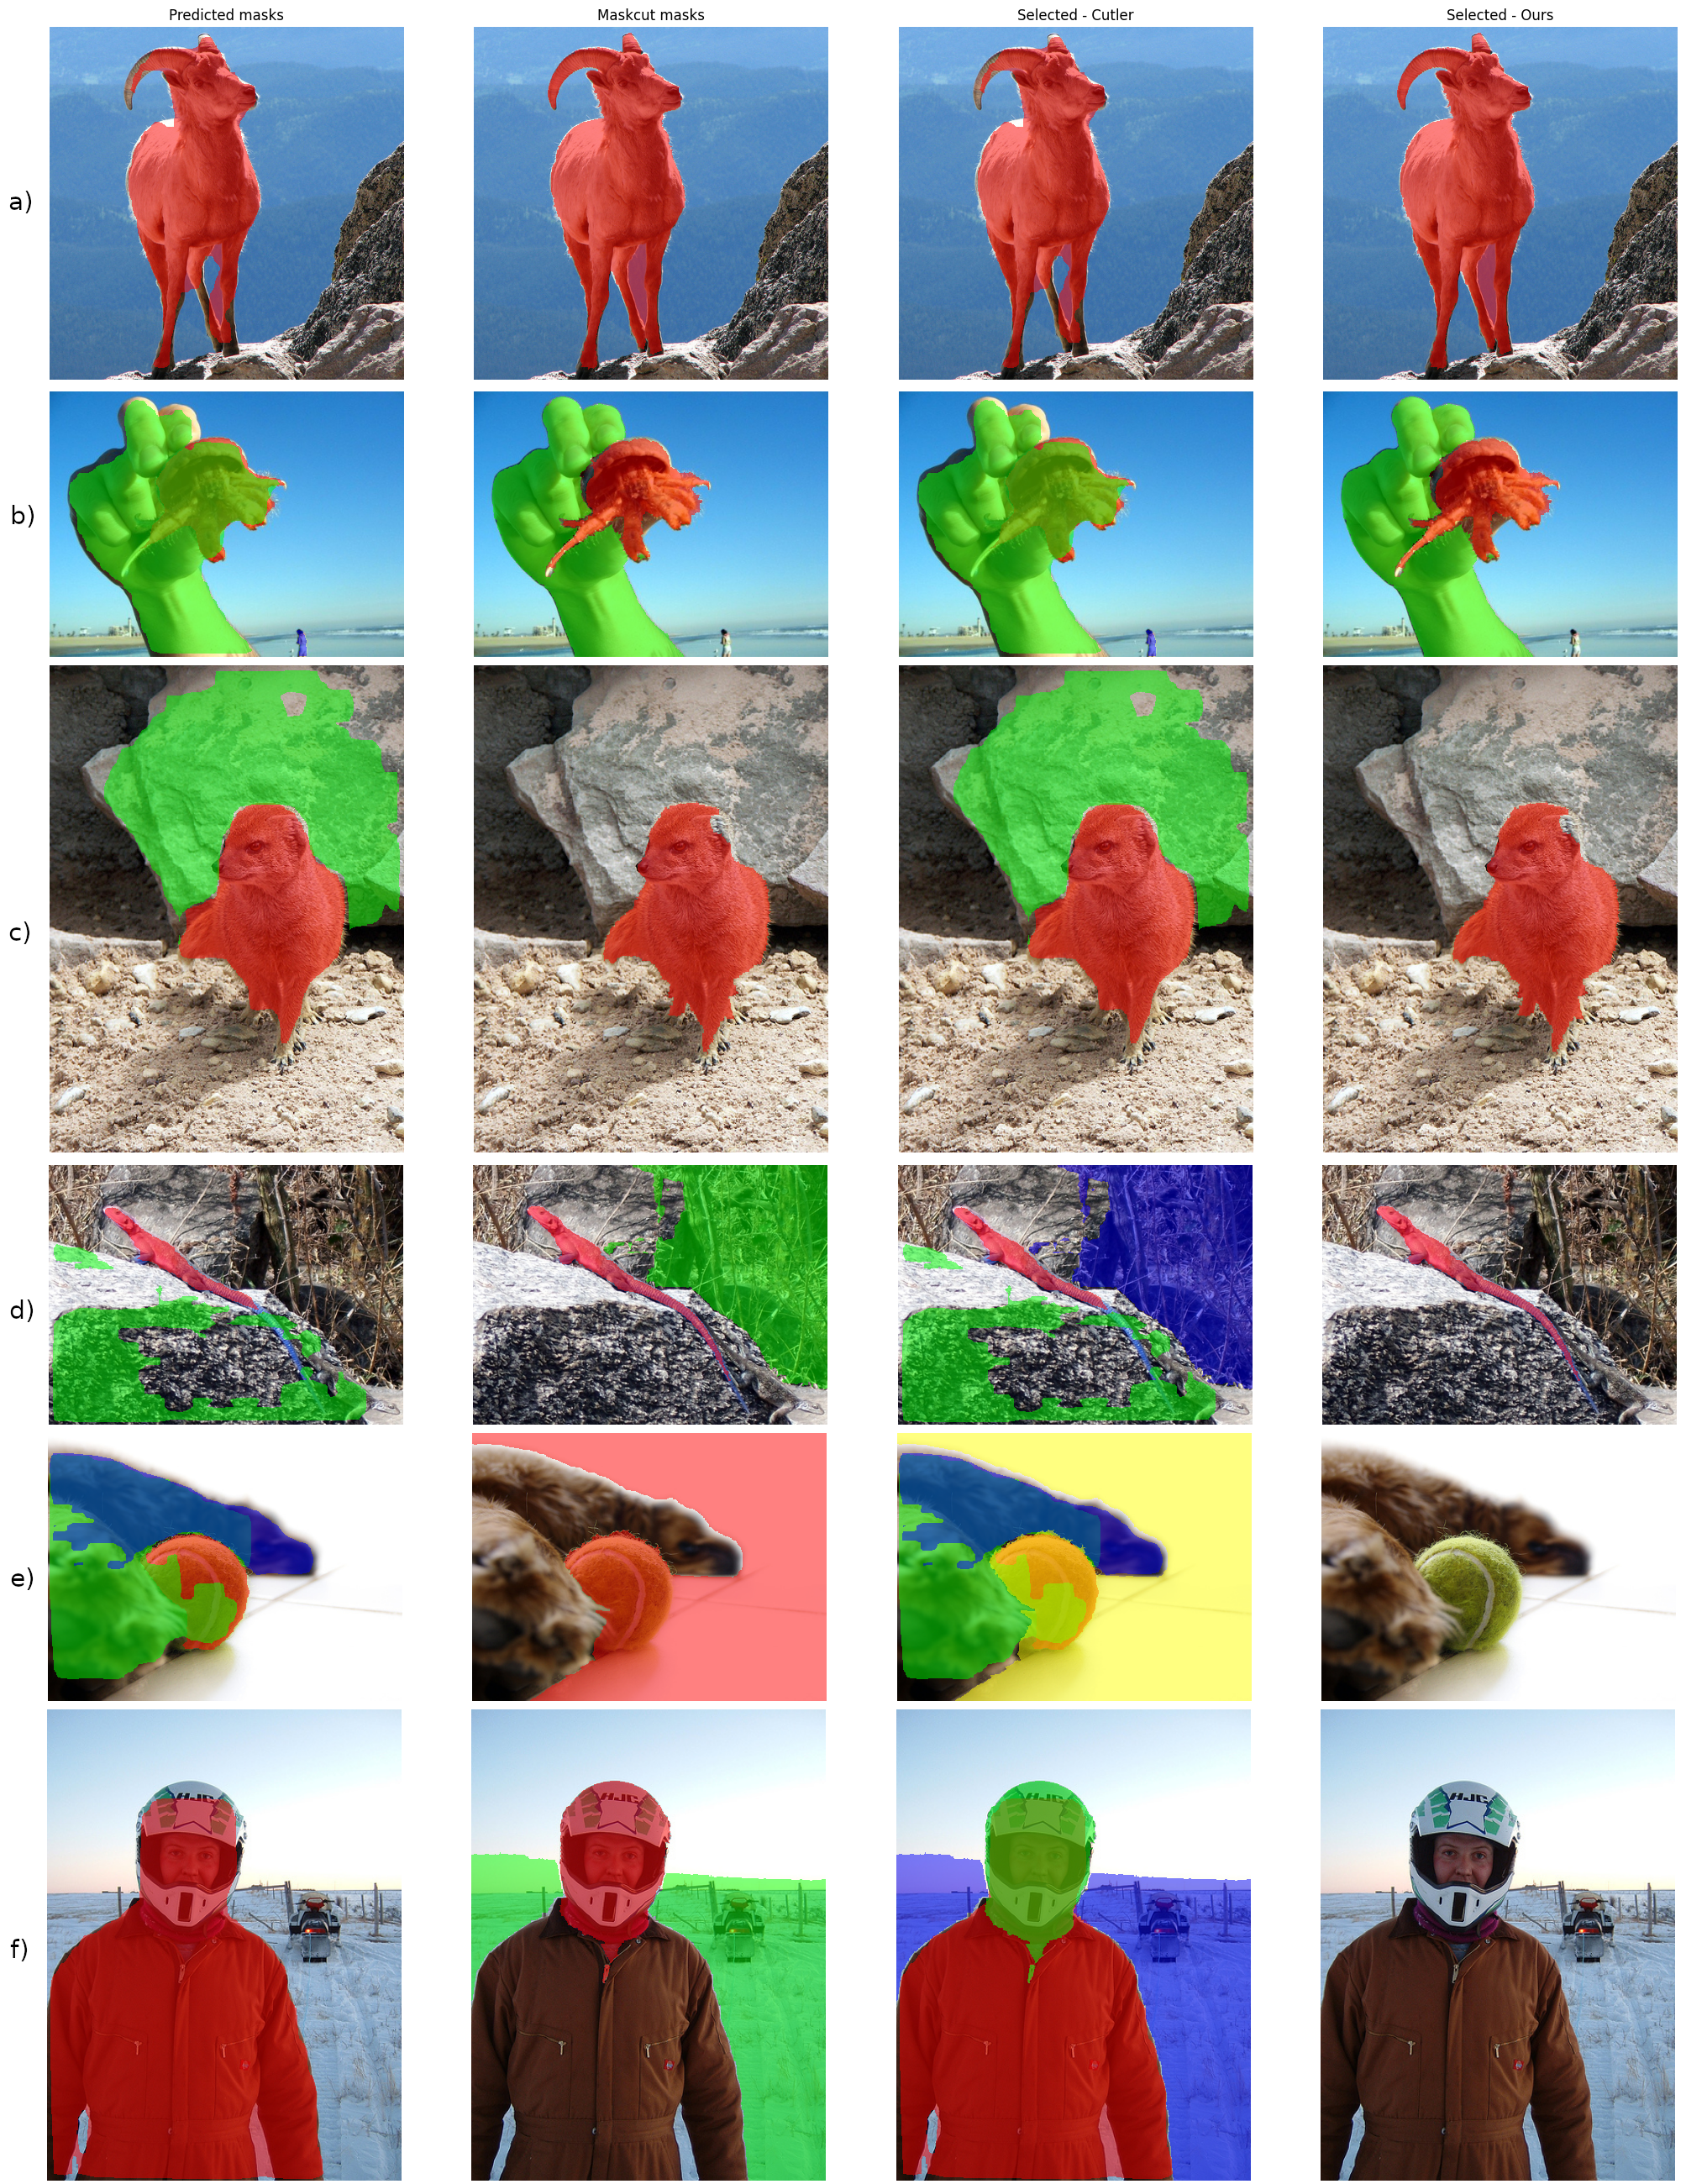
\includegraphics[width=1\textwidth]{Images/main/filtered_mask_comparison.png}
	\caption[\textbf{Mask Filtration Outputs - Baseline vs Ours}]{\textbf{Comparison of Filtered Masks} produced by the baseline and our method. Examples illustrates Cutler prediction masks, MaskCut masks, masks selected by CutLER and masks selected by our method respectively (left to right).}
	\label{fig:filtered_mask_comparison}
\end{figure*}
\begin{table}[htbp]
	\centering
	\resizebox{0.67\textwidth}{!}{%
	\begin{tabular}{c|cccc}
		\toprule
		Metric & AP & AP50 & AR1 & AR10 \\ \midrule
		MaskCut & 23.3 & 42.6 & 41.5 & 47.5 \\
		\midrule
		Our Mask Filtration & \textbf{28.3} & \textbf{50.3} & \textbf{44.4} & \textbf{48.0} \\
		\bottomrule
	\end{tabular}%
}
	\caption[\textbf{Quantitative Comparison of CutLER vs Proposed Mask Filtration Methods}]{\textbf{Quantitative Comparison of CutLER vs Our Proposed Filtration Methods} evaluated on annotated ImageNet subset using bounding box labels.}
	\label{tab:mask_filtration}
\end{table}

In this section, we evaluate the quality of pseudo-ground truth masks used for training the baseline (MaskCut masks) and our model (Refined MaskCut masks using our Approach~\ref{section:proposed_method}).

Table~\ref{tab:mask_filtration} shows a quantitative comparison of the masks used by the baseline and filtered by our approach. Both masks are evaluated on the annotated ImageNet subset using bounding box labels. It is important to note that we only use 15\% less masks compared to MaskCut masks used by the baseline. Still, we outperform MaskCut in all precision and recall metrics. 

We observe a significant improvement in precision metrics, driven by the removal of potentially inaccurate masks. Additionally, there is a slight gain in recall, suggesting that our filtration method is balanced enough to produce sufficient masks without excessively limiting coverage of the ground truth. We are using AR10 metric because the number of labels in the ImageNet dataset is consistently fewer than 10~\cite{deng2009imagenet} and MaskCut method generates a maximum of 3 masks per image.

\paragraph{Qualitative Examples}
Figure~\ref{fig:filtered_mask_comparison} illustrates the differences between the masks selected by our method and the baseline method across few example images. It is important to note that selected CutLER masks are used for the first stage of self-training in the baseline, whereas we only filter MaskCut masks, which is used for retraining from scratch.

For most images with single instances with distinguishable background, there are no significant differences between masks selected by baseline and our method as given in Fig.~\ref{fig:filtered_mask_comparison}~(a). Unfortunately a huge part of ImageNet dataset contains single instance object-centric images with simple backgrounds. Hence the improvement that we might obtain can be minimal. Nevertheless, our method works best for examples shown in Fig.~\ref{fig:filtered_mask_comparison}~(b-d). In Fig.~\ref{fig:filtered_mask_comparison}~(b-c) our approach successfully removes incorrect masks introduced by CutLER that are overlaid on better MaskCut masks. In Fig.~\ref{fig:filtered_mask_comparison}~(d), despite both MaskCut and CutLER containing noisy masks, our method effectively filters out these imperfections.

As we discussed earlier in Section~\ref{section:proposed_method}, some images are dropped from the training dataset for not having any selected masks. In Fig.~\ref{fig:filtered_mask_comparison}~(e), the image is dropped due to no selected masks, but CutLER prediction and mask selection are also bad. But in Fig.~\ref{fig:filtered_mask_comparison}~(f) CutLER selection is certainly better compared to predicted masks. But the image will be dropped in our method. These examples reaffirm that we compromise on quantity for quality in our approach. But nevertheless our method outperforms baseline even with lesser data.

\subsubsection{Self-Training Using Proposed Mask Filtration Strategy}

\begin{table}[htbp]
	\centering
	\resizebox{0.4\textwidth}{!}{%
		\begin{tabular}{c|c|cc}
			\toprule
			& & \multicolumn{2}{c}{COCO}  \\ \midrule
			& & AP & AP50 \\ \midrule
			\multirow{2}{*}{Train} & Baseline & 11.17 & 20.12  \\ 
			& Ours & \textbf{11.47} & \textbf{20.81}  \\ \midrule
			\multirow{2}{*}{r1} & Baseline & \textbf{11.70} & \textbf{21.15}  \\ 
			& Ours & 10.66 & 19.20 \\ \bottomrule
		\end{tabular}%
	}
	\caption[\textbf{\(AP_{box}\) and \(AP50_{box}\) for Initial Training and First Self-Training Round}]{\textbf{\(AP_{box}\) and \(AP50_{box}\) for Initial Training and Self-Training} evaluated on COCO validation set (Batch size 8) for model trained using our mask filtration during self-training.}
	\label{tab:combined_train_and_r1}
\end{table}

All our models use proposed initial mask filtration method. However, using our mask filtration method during self-training results in diminishing evaluation score. The results are illustrated in Table~\ref{tab:combined_train_and_r1}. This however was expected, as our masks are already less in number and more refined than baseline.

On the other hand, using masks generated by our mask filtration method for initial training and baseline mask filtration strategy for self-training yields better results than baseline. All the following experiments follow this combination of filtrations.

\subsubsection{Self-Training Using CutLER Mask Filtration Strategy}

In this section, we present how using masks generated by our mask filtration method for initial training and baseline mask filtration strategy for self-training outperforms the overall performance of the baseline. 

Our evaluations span across five datasets, COCO 2017 Evaluation, KITTI, VOC, Comic, and Watercolor, focusing on instance detection and segmentation tasks. We utilized the precision metric to measure the performance, providing a granular analysis of how our method impacts the accuracy of bounding box and segmentation predictions.

The results summarized in Table~\ref{tab:combined_train} demonstrate the performance of both the baseline and our proposed method across different stages of training: the initial training phase and subsequent self-training iterations (r1 and r2). This table provides a comprehensive comparison of the model’s effectiveness on various datasets, shedding light on the strengths and weaknesses of each approach throughout the training process.


\begin{table}[htbp]
	\centering
	\resizebox{1.05\textwidth}{!}{%
		\begin{tabular}{c|c|cc|cc|cc|cc|cc}
			\toprule
			& & \multicolumn{2}{c|}{COCO} & \multicolumn{2}{c|}{KITTI} & \multicolumn{2}{c|}{VOC} & \multicolumn{2}{c|}{Comic} & \multicolumn{2}{c}{Watercolor} \\ \midrule
			& & AP & AP50 & AP & AP50 & AP & AP50 & AP & AP50 & AP & AP50 \\ \midrule
			\multirow{2}{*}{Train} & Baseline & 11.17 & 20.12 & 4.79 & 10.27 & 19.98 & 36.26 & \textbf{11.80} & \textbf{28.39} & \textbf{14.67} & \textbf{35.60} \\ 
			& Ours & \textbf{11.47} & \textbf{20.81} & \textbf{6.28} & \textbf{13.48} & \textbf{20.24} & \textbf{36.56} & 10.81 & 26.50 & 14.00 & 35.27 \\ \midrule
			\multirow{2}{*}{r1} & Baseline & 11.70 & 21.15 & 6.60 & 14.19 & 19.56 & 36.81 & \textbf{11.05} & \textbf{27.53} & 12.92 & 33.45 \\ 
			& Ours & \textbf{11.94} & \textbf{21.65} & \textbf{8.21} & \textbf{18.49} & \textbf{20.24} & \textbf{37.95} & 10.80 & 27.40 & \textbf{15.37} & \textbf{37.74} \\ \midrule
			\multirow{2}{*}{r2} & Baseline & \textbf{11.02} & 20.32 & 6.73 & 15.02 & \textbf{18.06} & 35.09 & \textbf{9.90} & \textbf{25.36} & \textbf{13.59} & \textbf{34.31} \\ 
			& Ours & 10.81 & \textbf{20.47} & \textbf{7.69} & \textbf{17.04} & 17.93 & \textbf{35.24} & 8.94 & 22.74 & 12.06 & 30.02 \\ \bottomrule
		\end{tabular}%
	}
	\caption[\textbf{\(AP_{box}\) and \(AP50_{box}\) for Initial Training and Self-Training}]{\textbf{\(AP_{box}\) and \(AP50_{box}\) for Initial Training and Self-Training} evaluated on COCO validation set (Batch size 8) for model trained using our mask filtration for initial training and baseline mask filtration for self-training.}
	\label{tab:combined_train}
\end{table}

%\begin{table}[htbp]
%	\centering
%	\resizebox{1.05\textwidth}{!}{%
%		\begin{tabular}{c|c|cc|cc|cc|cc|cc}
%			\toprule
%			& & \multicolumn{2}{c|}{COCO} & \multicolumn{2}{c|}{KITTI} & \multicolumn{2}{c|}{VOC} & \multicolumn{2}{c|}{Comic} & \multicolumn{2}{c}{Watercolor} \\ \midrule
%			& & AP & AP50 & AP & AP50 & AP & AP50 & AP & AP50 & AP & AP50 \\ \midrule
%			\multirow{2}{*}{Train} & Baseline & 8.77 & 17.52 & 4.79 & 10.27 & 19.98 & 36.26 & \textbf{11.80} & \textbf{28.39} & \textbf{14.67} & \textbf{35.60} \\ 
%			& Ours & \textbf{8.83} & \textbf{17.72} & \textbf{6.28} & \textbf{13.48} & \textbf{20.24} & \textbf{36.56} & 10.81 & 26.50 & 14.00 & 35.27 \\ \midrule
%			\multirow{2}{*}{r1} & Baseline & 11.70 & 21.15 & 6.60 & 14.19 & 19.56 & 36.81 & \textbf{11.05} & \textbf{27.53} & 12.92 & 33.45 \\ 
%			& Ours & \textbf{11.94} & \textbf{21.65} & \textbf{8.21} & \textbf{18.49} & \textbf{20.24} & \textbf{37.95} & 10.80 & 27.40 & \textbf{15.37} & \textbf{37.74} \\ \midrule
%			\multirow{2}{*}{r2} & Baseline & \textbf{11.02} & 20.32 & 6.73 & 15.02 & \textbf{18.06} & 35.09 & \textbf{9.90} & \textbf{25.36} & \textbf{13.59} & \textbf{34.31} \\ 
%			& Ours & 10.81 & \textbf{20.47} & \textbf{7.69} & \textbf{17.04} & 17.93 & \textbf{35.24} & 8.94 & 22.74 & 12.06 & 30.02 \\ \bottomrule
%		\end{tabular}%
%	}
%	\caption[\textbf{\(AP_{segm}\) and \(AP50_{segm}\) for Training and Self-Training}]{\textbf{\(AP_{segm}\) and \(AP50_{segm}\) for Training and Self-Training} evaluated on COCO Eval dataset (Batch size 8)}
%	\label{tab:combined_train_segm}
%\end{table}

\begin{figure*}
	\centering
	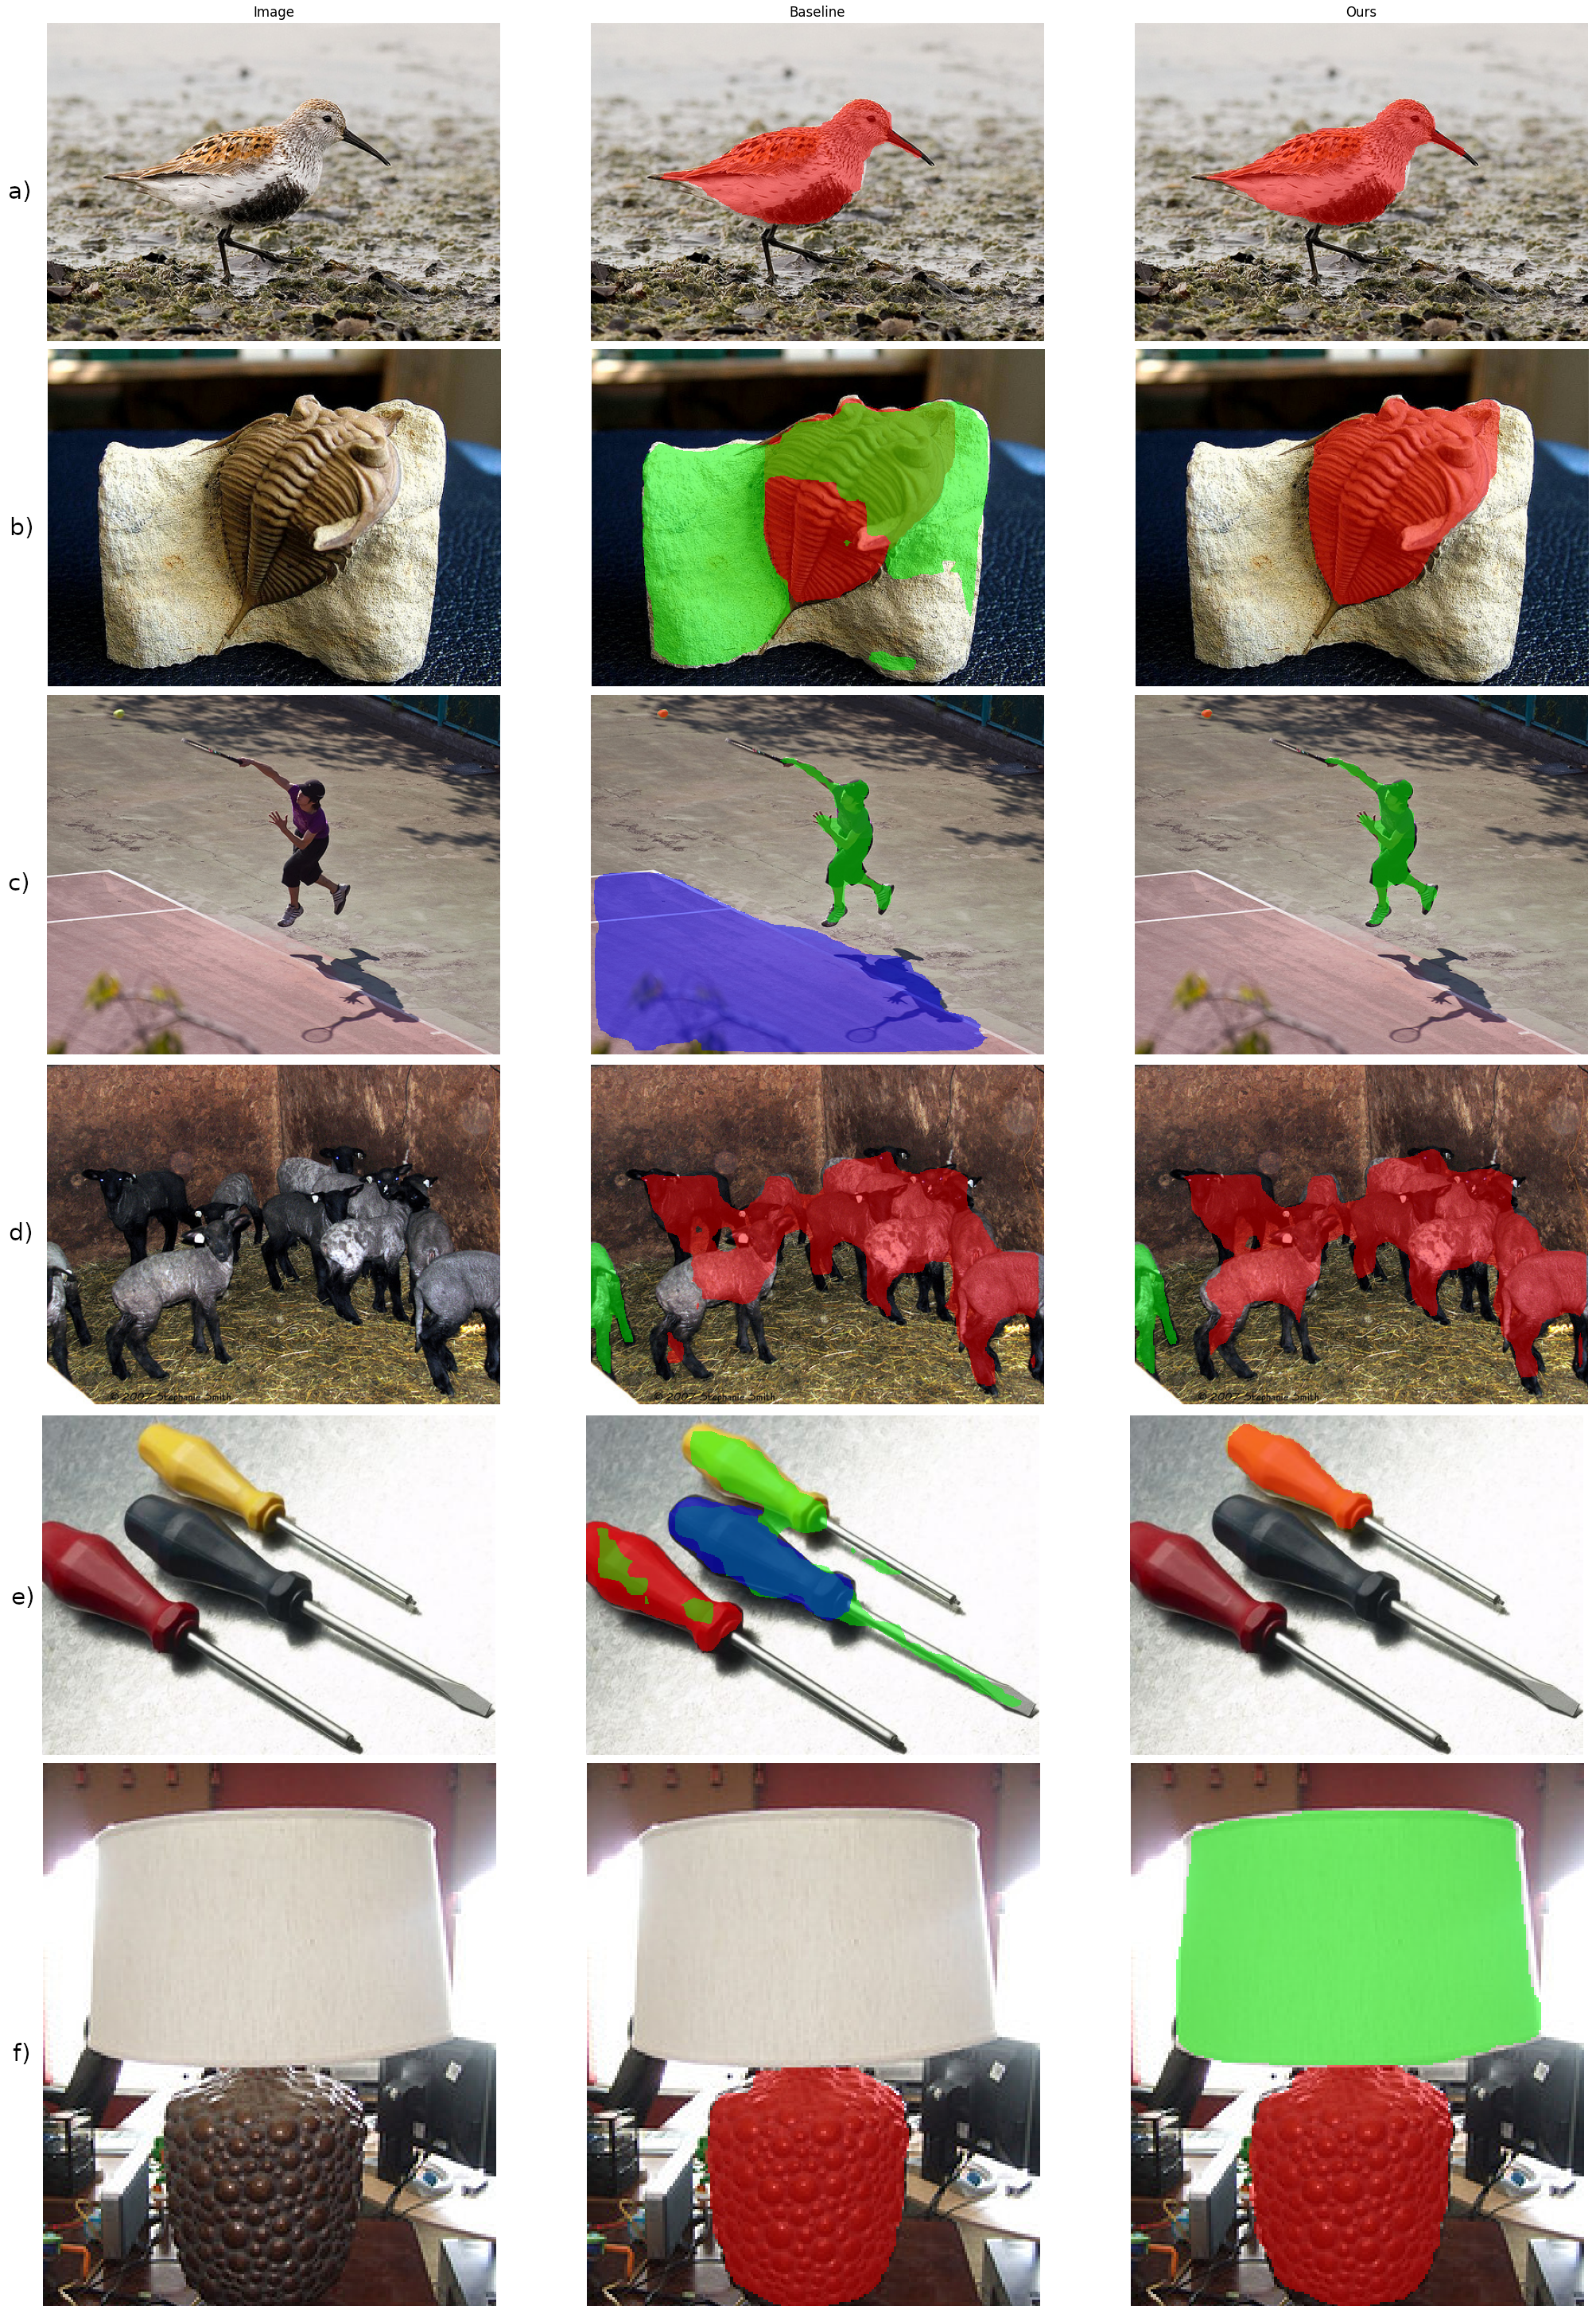
\includegraphics[width=1.05\textwidth]{Images/main/cutler_vs_ours.png}
	\caption[\textbf{Qualitative Results - Baseline vs Ours}]{\textbf{Qualitative Results - Baseline vs Ours} Masks predicted by CUtLER and Our model trained with modified mask filtration.}
	\label{fig:cuter_vs_ours}
\end{figure*} 

During the initial training phase, our method outperforms the baseline on the majority of the datasets, including COCO, KITTI, and VOC. Specifically, we observe a notable improvement in precision metrics, indicating that our refined mask filtration process is effective in enhancing the quality of pseudo-ground truths, leading to better detection and segmentation performance. However, our model slightly underperforms on the Comic and Watercolor datasets. After the first round of self-training, our model continues to outperform the baseline on 4 out of 5 datasets. In the second round of self-training, we observe a slight decline in performance across most datasets for both the baseline and our method, except for minor improvements in the baseline on the KITTI and Watercolor datasets. This decline could be attributed to the model’s diminishing returns from further self-training iterations due to more refined masks, especially when using smaller batch sizes, as noted in our experiments in Section~\ref{section:choice_of_batch_size}.

The evaluation on the Watercolor and Comic datasets has been somewhat inconsistent for both the baseline and our method. We hypothesize that this inconsistency arises from the stark difference between the types of images in these datasets compared to those in ImageNet. While our training predominantly involved real-life images, the Comic and Watercolor datasets consist of stylized, artistic images that pose a different challenge for the models. This disparity in image types likely contributes to the observed inconsistencies in performance.

\paragraph{Qualitative Results}

Figure~\ref{fig:cuter_vs_ours} presents a qualitative comparison between our method (with combination of mask filtration strategies for self-training) and the baseline. The predictions shown are generated using the most optimized models from both approaches, specifically after the first round of self-training.

Similar to the mask filtration method, for most images with single instances and distinguishable background, there is no significant difference between predicted masks by the baseline and our method as given in Fig.~\ref{fig:cuter_vs_ours}~(a). As our method is trained with a small number of filtered masks, our predictions mostly have lesser number of relatively better quality masks (Fig.~\ref{fig:cuter_vs_ours}~(b-c)). 

Grouping of the instances remains unsolved in both cases (Fig.~\ref{fig:cuter_vs_ours}~(d)). However, our method generates more complete masks with finer edges compared to the baseline. In Fig.~\ref{fig:cuter_vs_ours}~(e), our model doesn't predict any masks, but baseline model predicts 4 of them. It could be attributed to the conservative nature of our mask filtration method, predicting less, but higher confidence masks. However, there are few exceptions like Fig.~\ref{fig:cuter_vs_ours}~(f) where our model manages to predict more correct masks than the baseline. Even with this limitation, due to the improved quality of the masks, our method outperforms the baseline.
%
%\begin{table}[htbp]
%	\centering
%	\begin{tabular}{c|c|c|cl}
%		\toprule
%		Eval dataset & Imagenet-all & Imagenet-wo-ol & Imagenet-maskcut-filter \\
%		\midrule
%		Coco Eval & 10.35, 19.15 & 11.52, 20.67 & 11.44, 21.31 \\
%		\midrule
%		Coco Eval w/o overlapping inst. & 23.45, 38.11  & 24.77, 39.46 & 24.64, 40.64 \\
%		\midrule
%		Coco Eval only overlapping inst. & 7.25, 15.11 & 8.52, 16.8 & 8.32, 17.28 \\
%		\bottomrule
%	\end{tabular}
%	\caption{\textbf{AP and AP50 of evaluation(box) on COCO Eval datasets on models trained on imagenet for 90K iterations}}
%	\label{tab:ablationK}
%\end{table}
%
%\begin{table}[htbp]
%	\centering
%	\begin{tabular}{c|c|c|cl}
%		\toprule
%		Eval dataset & Imagenet-all & Imagenet-wo-ol & Imagenet-maskcut-filter \\
%		\midrule
%		Coco Eval & 7.87, 16.05 & 8.80, 17.47 & 9.1, 18.15 \\
%		\midrule
%		Coco Eval w/o overlapping inst. & 19.19, 35.19  & 20.13, 36.36 & 21.15, 38.31 \\
%		\midrule
%		Coco Eval only overlapping inst. & 5.12, 11.55 & 6.18, 13.27 & 9.78, 18.92 \\
%		\bottomrule
%	\end{tabular}
%	\caption{\textbf{AP and AP50 of evaluation(segm) on COCO Eval datasets on models trained on imagenet for 90K iterations}}
%	\label{tab:ablationK}
%\end{table}

\subsection{Choice of Batch Size}
\label{section:choice_of_batch_size}

\begin{table}[htbp]
	\centering
	\begin{tabular}{c|c|cc|cc}
		\toprule
		& & \multicolumn{2}{c|}{Batch size = 8} & \multicolumn{2}{c}{Batch size = 4} \\ \midrule
		& & AP & AP50 & AP & AP50 \\ \midrule
		\multirow{2}{*}{Train} & Baseline & 11.17 & 20.12 & 10.74 & 19.78 \\ 
		& Ours & \textbf{11.47} & \textbf{20.81} & \textbf{11.66} & \textbf{21.33} \\ \midrule
		\multirow{2}{*}{Self-train-r1} & Baseline & 11.70 & 21.15 & 11.35 & 21.23 \\ 
		& Ours & \textbf{11.94} & \textbf{21.65} & \textbf{11.79} & \textbf{21.58} \\ \midrule
		\multirow{2}{*}{Self-train-r2} & Baseline & \textbf{11.02} & 20.32 & 10.51 & 20.03 \\ 
		& Ours & 10.81 & \textbf{20.47} & \textbf{11.25} & \textbf{20.20 }\\ \bottomrule
	\end{tabular}
	\caption[\textbf{\(AP_{box}\) and \(AP50_{box}\) for Initial Training and Self-Training for Different Batch Sizes}]{\textbf{\(AP_{box}\) and \(AP50_{box}\) for Initial Training and Self-Training} evaluated on COCO validation set for batch sizes 4 and 8.}
	\label{tab:batch_size_table}
\end{table}

In the baseline paper, experiments were conducted using a batch size of 16. However, due to resource limitations, we performed our experiments with smaller batch sizes of 4 and 8. As shown in Table~\ref{tab:batch_size_table}, our results indicate a slight improvement in performance with a larger batch size, consistent with expectations that batch size can impact model performance.

Specifically, we observed that for both batch sizes of 4 and 8, the performance of our method and the baseline improved after the first round of self-training (r1) but declined in the second round (r2). This pattern diverges from the findings in the baseline paper, where using a batch size of 16 led to continued performance improvement through the second round of self-training. The observed performance drop in the second self-training round at smaller batch sizes suggests that batch size plays a crucial role in stabilizing the training process, potentially by providing more robust gradient estimates or better generalization.

Furthermore, the influence of batch size on the relative gains achieved through self-training is evident in our experiments. Larger batch sizes tend to offer a more stable training environment, which may explain the continued improvement seen in the baseline paper with a batch size of 16. Conversely, the smaller batch sizes used in our experiments may introduce greater variance, leading to less consistent performance gains across self-training rounds. This highlights the importance of considering batch size as a key factor in optimizing training pipelines for tasks involving self-training and iterative refinement.

\subsection{Impact on Recall}
\label{section:persistant_recall}

\begin{table}[htbp]
	\centering
	\resizebox{0.85\textwidth}{!}{%
		\begin{tabular}{c|c|c|c|c|c|c}
			\toprule
			& & COCO & KITTI & VOC & Comic & Watercolor \\ \midrule
			\multirow{2}{*}{Baseline} & bbox & \textbf{32.06} & 25.91 & \textbf{43.70} & 36.97 & 42.30 \\ 
			& segm & 26.16 & - & - & - & - \\ \midrule
			\multirow{2}{*}{Ours} & bbox & 31.75 & \textbf{26.41} & 43.34 & \textbf{38.24} & \textbf{43.46} \\ 
			& segm & \textbf{26.44} & - & - & - & -
			\\ \bottomrule
		\end{tabular}%
	}
	\caption[\textbf{\(AR_{100}\) for the Best Models of the Baseline and Our Method}]{\textbf{\(AR_{100}\) for the Best Models of the Baseline and Our Method} (Models from the First Self-Training Round) evaluated on COCO validation set for segmentation (segm) and detection (bbox) tasks.}
	
	\label{tab:recall}
\end{table}

Average Recall (AR) is a valuable metric for unsupervised detection as it does not penalize the models for detecting novel objects which are unlabeled in the dataset. In our case, as our method only produces less number of masks than the baseline, a small reduction in recall was expected. However, it has not affected to the scale we had expected.

Table~\ref{tab:recall} shows \(AR_{100}\) for the best models of our method and the baseline evaluated over 5 different datasets. We observe that our model outperforms the baseline across three datasets, while achieving results that are very close in the remaining two. This suggests that our approach focused on improving precision has had minimal impact on recall.

